\chapter{Panel operatora procesu}
\label{thermal_panel}
Na panelu operatora wyświetliliśmy możliwie najprościej najważniejsze informacje na temat obiektu tj. wielkość mierzoną i zadaną wyjść procesu oraz wartości sterowań. Zamiast długich opisowych nazw użyliśmy krótkie, ale zarazem jednoznaczne, dzięki czemu operator skupia się głównie na wyświetlonych wartościach liczbowych, a nie na odczytywaniu nazw. Panel HMI został zaprojektowany zgodnie z najnowszymi standardami stosowanymi w przemyśle. Skupiają się one głównie na czytelności panelu, dlatego stosuje się m. in. odcienie szarości czy też zgromadzenie informacji, które mają ze sobą coś wspólnego w jednym obszarze. Oznaczenie użyte na panelu prezentują się następująco, \textit{STPT1}, \textit{STPT2} to aktualna wartość zadana dla danego wyjścia, \textit{U1}, \textit{U2} to aktualne sterowanie, a \textit{Y1}, \textit{Y2} aktualne wyjście procesu. 

\begin{figure}[H]
\setlength{\leftskip}{-0.2cm}
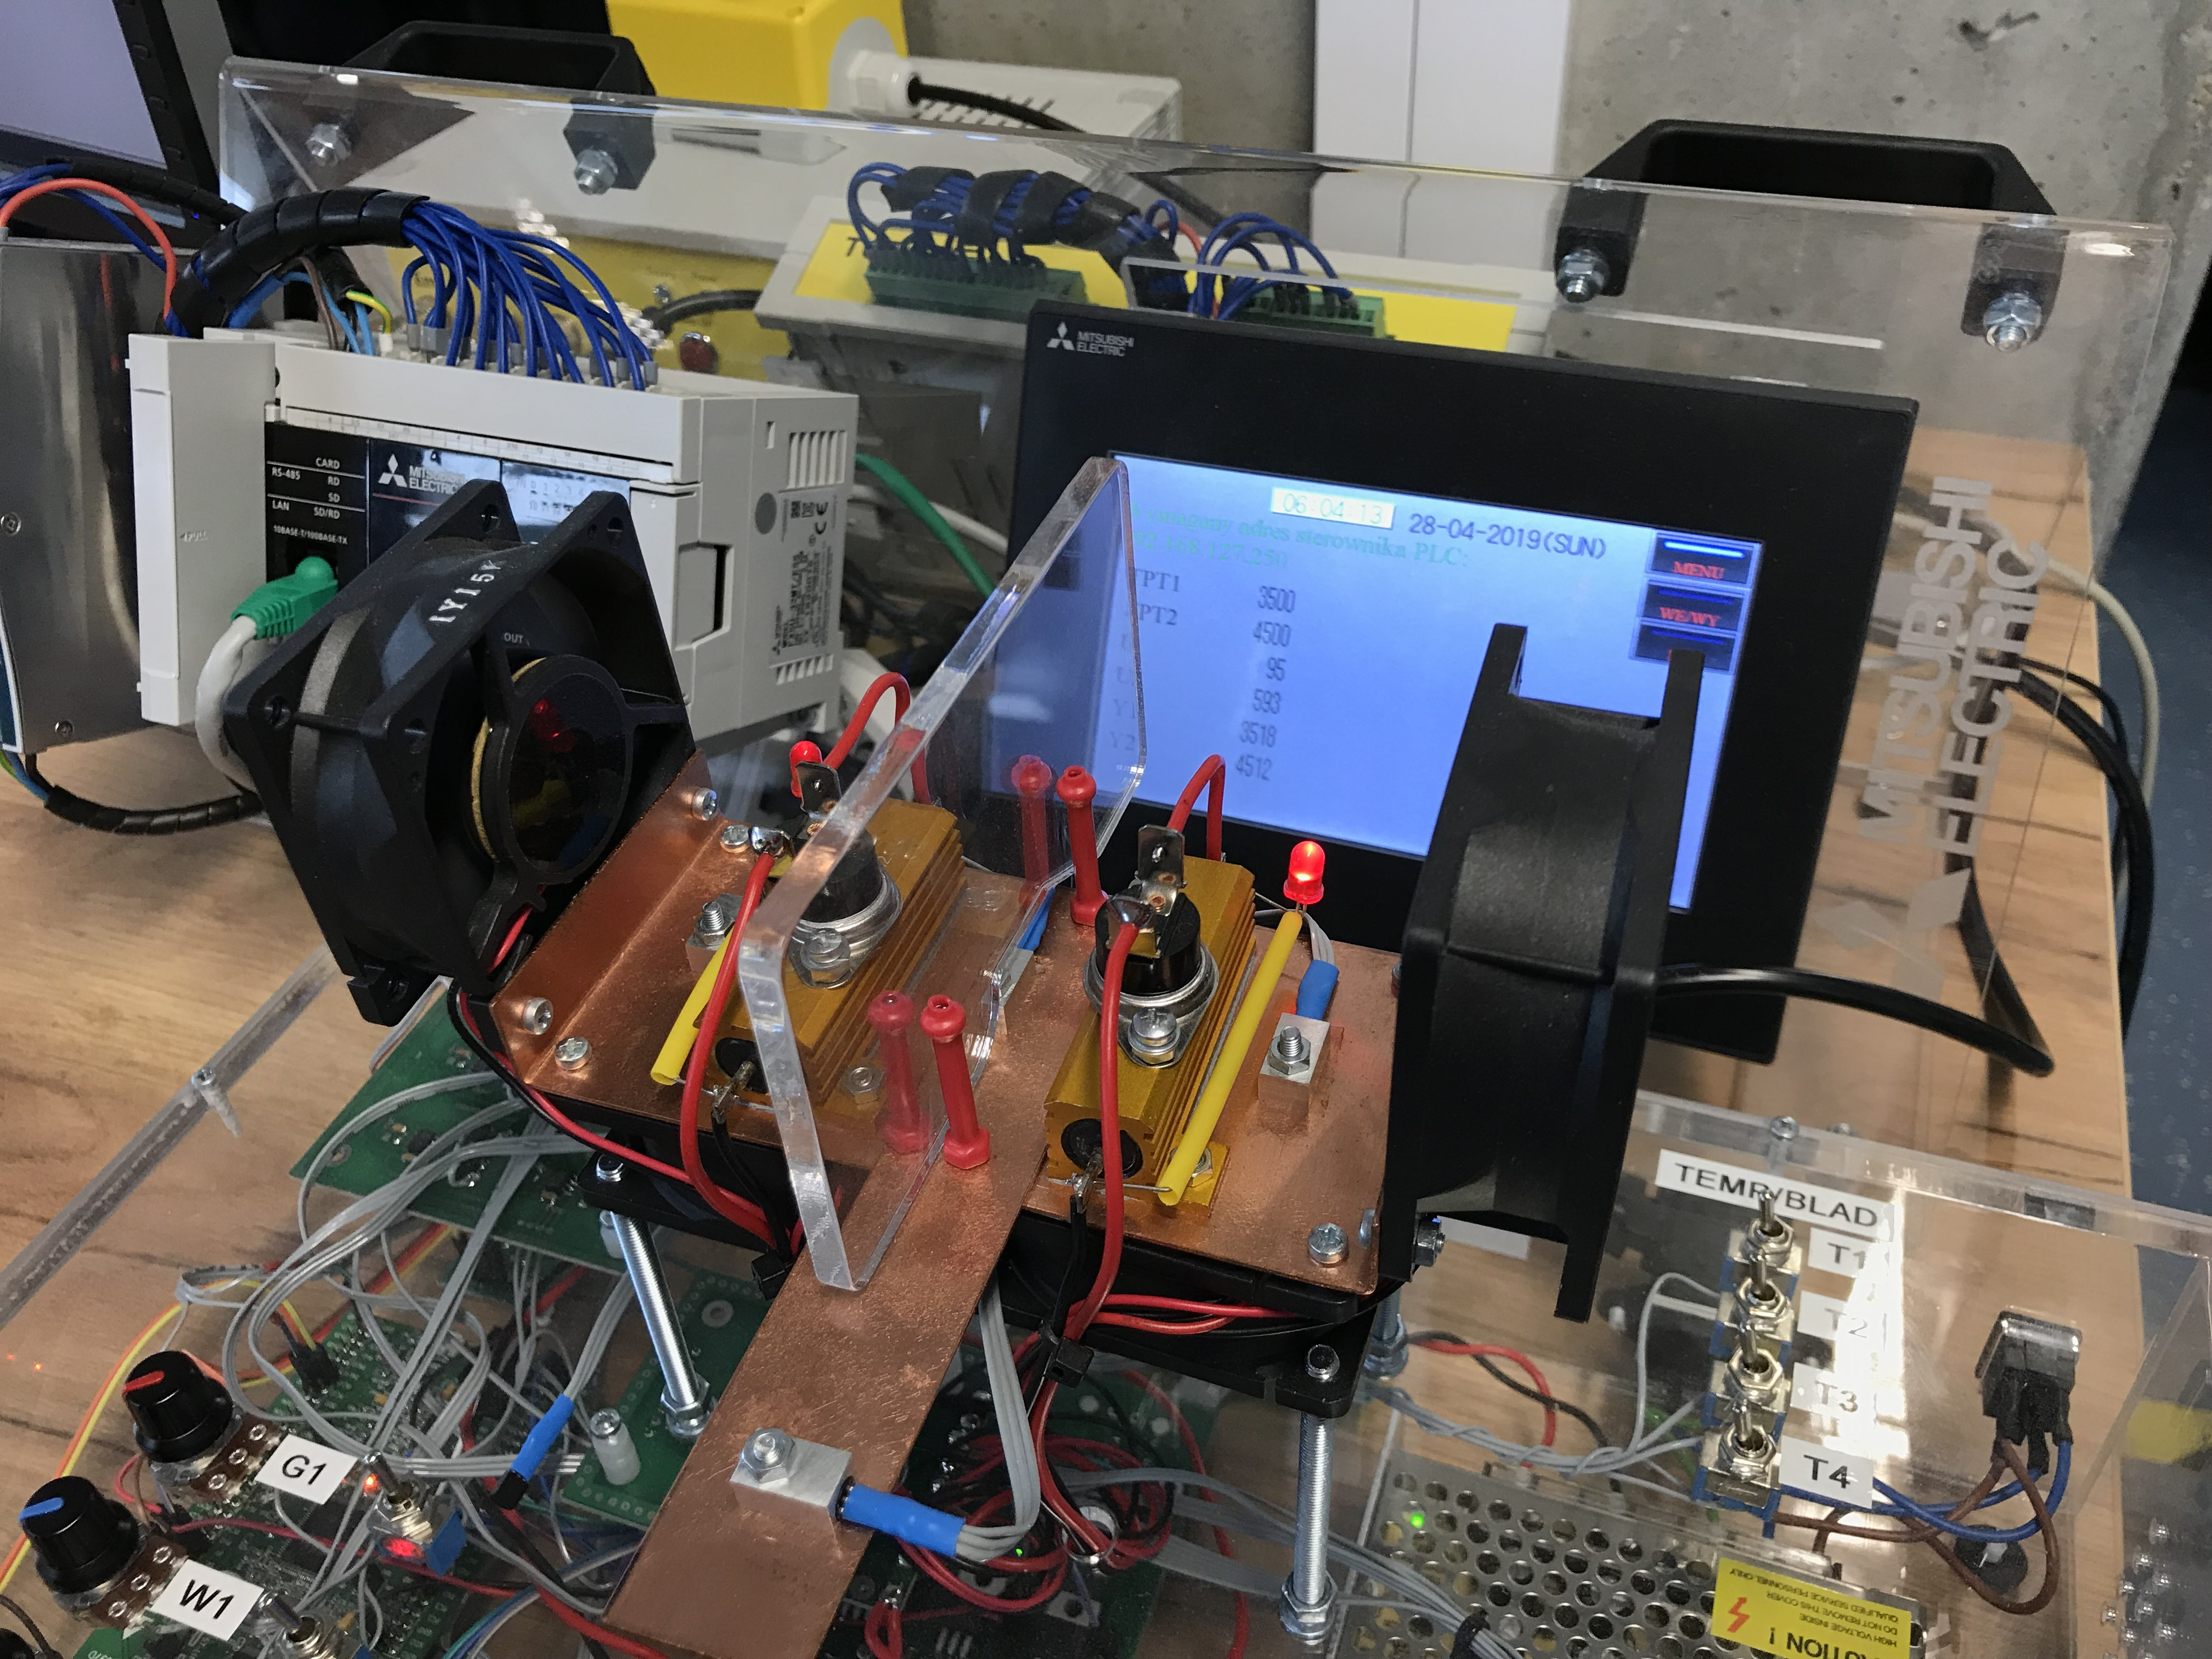
\includegraphics[scale=0.09]{../data/lab/thermal_object/zad5/IMG_0964.JPG}
\caption{Pracujące stanowisko chłodząco-grzejące z działającym w tle panelem operatorskim}
\end{figure}

\begin{figure}[H]
\setlength{\leftskip}{-0.2cm}
\includegraphics[scale=0.09]{../data/lab/thermal_object/zad5/IMG_0965.JPG}
\caption{Panel operatorski pokazujący aktualne dane z zachodzącego procesu regulacji}
\end{figure}

\begin{figure}[H]
\setlength{\leftskip}{-0.2cm}
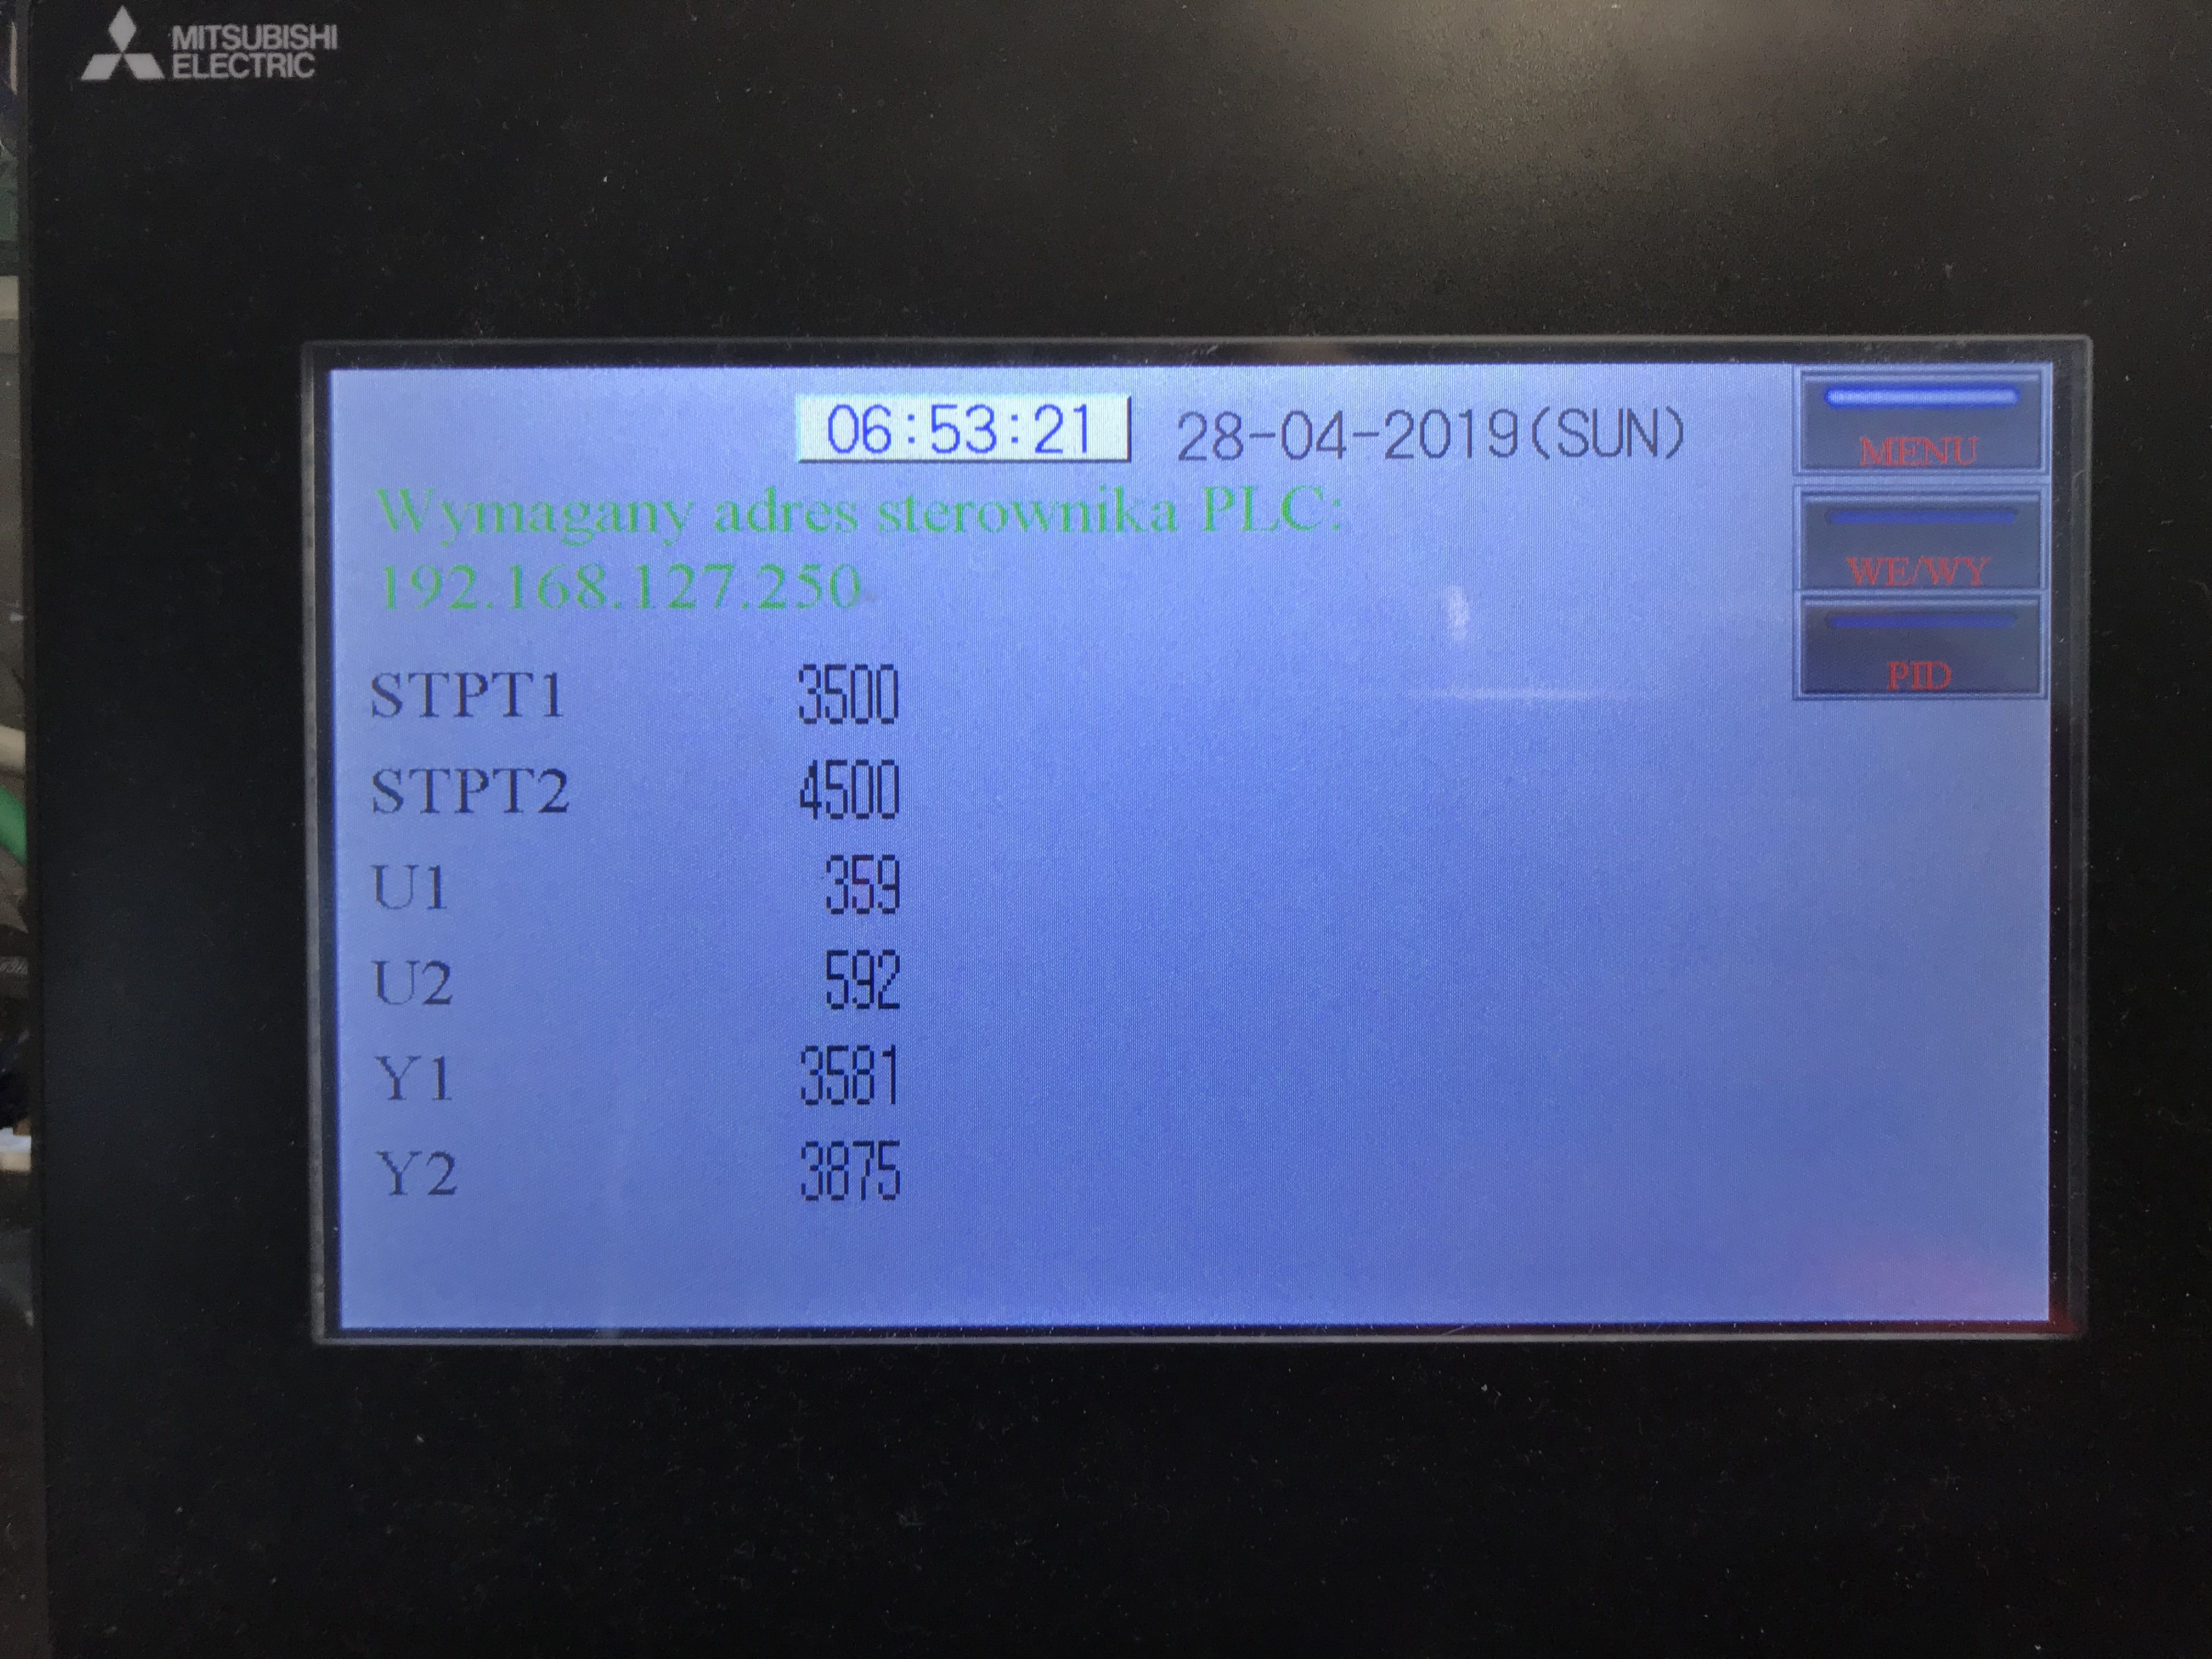
\includegraphics[scale=0.09]{../data/lab/thermal_object/zad5/IMG_0966.JPG}
\caption{Panel operatorski pokazujący aktualne dane z zachodzącego procesu regulacji}
\end{figure}